% Created 2018-05-15 二 01:04
\documentclass[fontset=windows,11pt]{ctexart}
\usepackage[utf8]{inputenc}
\usepackage[T1]{fontenc}
\usepackage{fixltx2e}
\usepackage{graphicx}
\usepackage{longtable}
\usepackage{float}
\usepackage{wrapfig}
\usepackage{rotating}
\usepackage[normalem]{ulem}
\usepackage{amsmath}
\usepackage{textcomp}
\usepackage{marvosym}
\usepackage{wasysym}
\usepackage{amssymb}
\usepackage{hyperref}
\tolerance=1000
\usepackage{listings}
\usepackage{minted}
\date{2018-05-08}
\title{文字识别探索}
\hypersetup{
  pdfkeywords={},
  pdfsubject={},
  pdfcreator={Emacs 25.3.1 (Org mode 8.2.10)}}
\begin{document}

\maketitle
\tableofcontents


\section{前言}
\label{sec-1}
目前Guacamole的图形审计功能只能做到基础的回放,以及根据会话的信息进行简单检索·\footnote{其实也没有显示支持,不多可以通过一些取巧的做法完成。}。跟字符协议不同,图形协议传输的数据主要是桌面图片(实际上不是,方便起见先这么理解)。图片只适合人工处理,初步能人工处理
这里为了方
一份数据足矣
\section{OCR功能}
\label{sec-2}
 OCR(optical character recognition,光学字符识别),是指电子设备(例如扫描仪或数码相机)检查纸上打印的字符,通过检测暗、亮的模式确定其形状,然后用字符识别方法将形状翻译成计算机字符的过程。
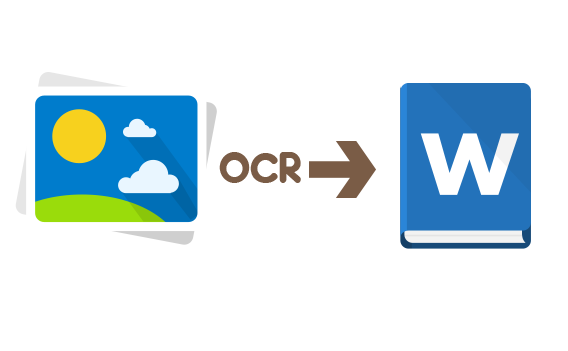
\includegraphics[width=.9\linewidth]{./文字识别探索/ocr-to-word.png}

OCR是一个多学科交叉领域,涉及到计算机视觉(图像处理)、模式识别、机器学习和神经网络等方面知识,属于一个很复杂的领域。一般OCR主要分成了两步:
\begin{enumerate}
\item 文字提取
\item 文字识别
\end{enumerate}

其中文字提取的繁杂度远远高于文字识别\footnotemark[1]{}。

由于RDP已经帮我们提取了一部分文字,这部分文字位图相当于已经完成了文字提取后的位图数据,这部分数据可以比较高效地被文字识别软件识别,
多数实现了文字审计的堡垒机厂家都避开了文字提取的部分,或者只进行简单的处理。这样就导致了没有办法进行高质量全文搜索的。如果使用这一部分数据
 实际上RDP已经帮我们提取了一部分文字,只要在guacd的RDP模块中截取这一部分数据就可以用于识别了,除此之外还有一部分文字由于不是由Window进行渲染所以只能以图片的形式传输,这里的文字提取主要就是指的这种情况。多数堡垒机的OCR功能都没有处理这一部分数据。也就是说并没有进行文字提取。
\subsection{文字识别范围的选择}
\label{sec-2-1}
对于RDP的文字识别,主要涉及两个范围:
\begin{enumerate}
\item 通过RDP的传输文字
\item 除此之外图像中的文字
\end{enumerate}

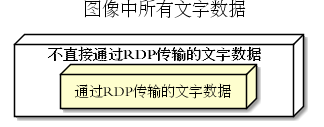
\includegraphics[width=.9\linewidth]{文字识别探索/cover.png}



只识别通过RDP传输的字体和识别整幅图像的字体这两种选择带来的难度差异巨大,这也是为什么几乎没有堡垒机识别整幅图像的文字。因为作出这个选择的代价十分巨大,而且能带来的收益只是全文检索效果的上升。就目前看来哪怕是全文检索的需求都不算很大。
\subsection{Tesseract-OCR}
\label{sec-2-2}
得益于通过RDP传输的文字都是都是某种字体的字形数据,这个正好就是Tesseract原本使用的领域,所以识别率很不错。只是识别通过RDP传输的文字倒是没有遇到什么麻烦。   
\section{历史记录检索}
\label{sec-3}
说到检索,最简单的方式当然是把数据集合放到内存中遍历一遍,如果发现消耗的时间或者内存不可接受,就可以考虑使用数据库或者其他的某些检索库。一般数据库重点在于解决后者:内存不足问题。
\subsection{Guacamole历史文件格式介绍}
\label{sec-3-1}
\subsubsection{基本逻辑}
\label{sec-3-1-1}

\subsubsection{当前可以用于实现的功能}
\label{sec-3-1-2}
\subsubsection{前端的工作}
\label{sec-3-1-3}
\subsection{中文分词}
\label{sec-3-2}
\subsection{检索需求介绍}
\label{sec-3-3}
说到检索,最简单的方式当然是把数据集合放到内存中遍历一遍,如果发现消耗的时间或者内存不可接受,就可以考虑使用数据库或者其他的某些检索库。一般数据库重点在于解决后者:内存不足问题。
历史记录检索功能根据范围主要分成三类:
\begin{enumerate}
\item 单个历史记录的检索
\item 小数量级的多个历史记录的检索
\item 大数量级的多个历史记录的检索
\end{enumerate}

单个历史记录的检索是最简单的,由于数据量不大,可以采用直接放到内存中遍历一遍的方式,推荐直接在前端完成。如果是查询某个用户在某段时间内的操作历史这一类的小数量级的检索,也可以直接由前端在获取所有数据文件之后遍历检索,开销也可以接受。最大的难点还是在于大数量级的多个历史记录的检索,这个涉及 \textbf{全文检索} 领域。
应用场景
\subsection{全文搜索}
\label{sec-3-4}
全文搜索是一种数据模型,常常被用在数据库中。支持全文检索模型的软件包括PostgreSQL、MySQL、MongoDB、levelDB这类比较常用的数据库。之所以可以和各种数据库结合,主要原因是这个数据模型本身比较独立,不会和其他数据模型发生冲突。
全文检索的主要用于高效查询关键字,一旦开了索引,那么就需要在插入新数据的时候维护索引数据结构,插入的开销会随之增大。
\subsubsection{检索的基本原理}
\label{sec-3-4-1}
\subsubsection{全文检索和键值检索}
\label{sec-3-4-2}
关系数据库默认情况下提供了基础的键值检索功能,根据键可以高效地找到相应的记录,根据键可以查找。
\subsubsection{Apache Lucene}
\label{sec-3-4-3}
Lucene是Elasticsearch和Solr使用的一种全文搜索的索引引擎。它一个完成度很高的软件,在全文检索的领域也是比较出名的软件。当然它是一个框架,不算一个应用软件,要测试其效果可以尝试一下基于它的两个比较出名的软件是:
\begin{enumerate}
\item DocFetcher
\item Apache solr
\item Nutch
\end{enumerate}

通过简单定制和优化可以满足上亿级别的检索,同时也支持分布式。之所以需要分布式,主要是全文检索本身是一个开销极大的功能,使用关系数据库的全文检索功能的时候也要小心对数据库性能造成影响。
由于Lucene是使用Java编写的软件,所以基于Lucene的项目大多也是Java项目。当然,Python可以通过使用PyLucene来使用Lucene。
\subsubsection{针对Guacamole历史文件的搜索引擎设计}
\label{sec-3-4-4}
很多检索工具都是基于Lucene进行索引的根据具体
\subsubsection{Guacamole}
\label{sec-3-4-5}
\subsection{数据库的使用原因}
\label{sec-3-5}
其实数据库解决的是海量数据的存储问题,首先,一旦涉及海量数据,直接靠在内存中遍历的所有数据的方式已经不可能了,除了运行时间的问题还有内存的限制。为了解决这两个问题才有了数据库。数据库做到了我们获取数据的时候一次只有少数的数据滞留在内存中。并不是关系模型对于处理数据有无以比拟的优势。

\section{针对特定模式的处理}
\label{sec-4}
首先,我们知道通过图形界面(GUI)是无法完全获知程序内部逻辑的,这个结论决定图形审计的上限。所以要为图形审计添加功能,就只能 \textbf{从能够获取的数据中不断挖掘出特定的“模式”} 。各家堡垒机做的事情无非就是如此,区别只在于挖掘到或者设计的“模式”多少的问题。
\subsection{文字审计}
\label{sec-4-1}
例如,行云管家提取出了通过RDP传输的文字之后,为此设计的“模式”叫做指令,指令被分成以下四种:
\begin{itemize}
\item 窗口
\item 菜单
\item CMD
\item 其他
\end{itemize}
以上。。。当然这种区分似乎有点超前了,可能是先设计了“模式”,再来挖掘“模式”造成,也可能是只注意到某些特例,并为这些特例设计的“模式”。适用范围有限。
\subsection{键盘审计}
\label{sec-4-2}
这里先用键盘审计举例:
各家键盘审计价值其实都没有那么大,键盘的处理如果小到单个按键这个粒度(OEM堡垒机),几乎不具备可用性,就像没人看英文会一个个字母看一样,至少要到单词这个粒度。当然现实没那么绝望,即使是单个按键的层面也不是不能找到”模式“,比如PrintScreen键,单个按键就足以表达”打印屏幕“这个语义了。
\subsection{按键“模式”}
\label{sec-4-3}
处理用户按键信息的情况也类似,由于本身信息不足,想进一步也是挖掘“模式”。单独处理按键信息其实很局限,路很快就走死了(毕竟就那点信息,类似OEM干脆把所有按键信息列出来)。出路大概就是和文字信息结合起来进行“模式“挖掘。
\section{总结}
\label{sec-5}
目前看来,为了提升图形审计效果,大体上就是两个方向:
\begin{enumerate}
\item 增强从图像中提取的数据的能力(不单包括文字)
\item 不断从获取的数据中发现更多”模式“
\end{enumerate}

历史记录的检索效果则取决于能第一个方向走多远。数据量越大,检索的价值也越大。检索性能优化的空间则非常有限,全文检索算是非常成熟的技术了。
\section{零散}
\label{sec-6}
\begin{itemize}
\item 最小改动原则
\item 图像改动原则
\item 试试播放的时候并没有开ocr,似乎是为了
\end{itemize}
\section{参考}
\label{sec-7}
\begin{itemize}
\item 《设计及数据密集型应用》
\end{itemize}
% Emacs 25.3.1 (Org mode 8.2.10)
\end{document}